Omega3P is a C++ component within ACE3P for frequency analysis
of linear accelerator cavities~\cite{ko2010advances}.
It is built upon multiple components that include distributed mesh
functionality (DistMesh), tensor field management, vector and
matrix math, and many linear solvers.
Our in-memory integration of PUMI with Omega3P leverages these APIs to execute
bulk mesh and field transfers, and atomic element Jacobian transfers for element
stiffness matrix formation.

In the previous section we discussed a similar in-memory integration
for efficient parallel adaptive workflows with Albany.
In Omega3P, as with Albany, we again assume a small increase in memory
usage from storing both the PUMI mesh and Omega3P DistMesh.
This small memory overhead lets us avoid spending time destroying and reloading
the PUMI mesh after the adaptation and analysis steps, respectively.
Furthermore, having access to the PUMI mesh supports the atomic transfer of exact
geometry of curved domains needed for calculation of mesh element Jacobians
during element stiffness matrix formation.
This capability is critical in Omega3P for maintaining convergence of higher
order finite elements when the geometric model has higher order curvature
~\cite{DeyShephard_97,LuoShephard_02,LuoShephard_04}.

Algorithm~\ref{alg:omega3pJacobian} lists the steps needed to compute the exact
Jacobian using the APF \texttt{getJacobian(...)} API and its underlying
basis functions.
To set up this process a pointer to each PUMI mesh element is stored
with the corresponding DistMesh element object as they are being
created during the PUMI-to-DistMesh conversion.
As the DistMesh elements are being traversed for element stiffness
matrix assembly the PUMI element pointer is retrieved
($l.$\ref{alg:o3p_pointer}).
With this pointer and the barycentric coordinates of the element
($l.$\ref{alg:o3p_bary}) the 3x3 Jacobian matrix is computed by the call to the
APF \texttt{FieldShape} \texttt{getJacobian} function ($l.$\ref{alg:o3p_getJ}).

% 62842e2 of the SCOREC/ace3p branch geom_inquiries
% hierarchical(...) calls assemblePatternValue in loop over element container
% emfem/src/MatrixAssemblyHierarchical.h +150
%   ^ calls updateMatrices
%   emfem/src/MatrixAssemblyHierarchical.h +205
%     ^ calls elementalMatrices
%     emfem/src/MatrixAssemblyHierarchical.h +49
%       ^ calls calculateDxDyDzLambda in loop over integration points
%       emfem/src/HierarchicalElement.C +214
%         ^ calls calculateInverseJacobian
%         emfem/src/HierarchicalElement.C +237
%           ^ calls calculateBaryCentricJacobian
%           emfem/src/O3P_Element.C +401
% We don't directly call getJacobian(...) in O3P_Element.C as there
%  is some local coordinate transformation work that needs to be done.
%  But, we still call the getLocalGradients(...) function which is a
%  member of the 'shape' associated with the element, which is what
%  getJacobian(...) does internally.
\begin{algorithm}
  \caption{Jacobian Calculation for Matrix Assembly}
  \label{alg:omega3pJacobian}
  \begin{algorithmic}[1]
    \State // loop over DistMesh elements
    \ForAll{ $M^3_i \in \{M^3\}$ }
      \State $pumiElementPtr \gets getPumiElementPtr(M^3_i)$
             \label{alg:o3p_pointer}
      \ForAll{ integration points }
        \State // compute element Jacobian using
                  APF's \texttt{FieldShape} class
        \State // associated with the PUMI mesh element
        \State $xi \leftarrow$ getBaryCentricCoords(integration point)
               \label{alg:o3p_bary}
        \State \texttt{apf::Matrix3x3} $J$
        \State \texttt{apf::getJacobian($pumiElementPtr$,$xi$,$J$)}
               \label{alg:o3p_getJ}
        \State // complete element matrix computation
      \EndFor
      \State // insert element matrix contributions into stiffness matrix
    \EndFor
  \end{algorithmic}
\end{algorithm}

The mesh management and computational steps in the adaptive Omega3P-PUMI
workflow are listed in Algorithm~\ref{alg:omega3pAdaptLoop}.
Fig.~\ref{fig:omega3pAdapt} depicts adapted meshes and fields generated using
this process.
Execution of the workflow begins by loading a distributed PUMI mesh
and the geometric model ($l.$\ref{alg:o3pPumiLoad}-\ref{alg:o3pGeom}).
Next, ParMA balances the owned and ghosted mesh
entities holding degrees of freedom (edges and faces for quadratic Nedelec shape
functions~\cite{ingelstrom2006new}) ($l.$\ref{alg:o3pParma1}).
PUMI APIs are then used to create a DistMesh instance from the balanced PUMI
mesh ($l.$\ref{alg:o3pDistMesh}); a bulk transfer.
The time required for this procedure is less than 0.1\% of the total workflow
execution time.
Next, the workflow runs the solve-adapt cycle until the eigensolver has
converged ($l.$\ref{alg:o3pWhile}).
Note, the atomic Jacobian transfer of Algorithm~\ref{alg:omega3pJacobian} occurs
during the eigensolver execution.
Following the solver's execution the electric field is attached to the PUMI
mesh ($l.$\ref{alg:o3pGetField}) via a bulk transfer, the DistMesh is destroyed
($l.$\ref{alg:destroyDistmesh}),
a size field is computed by SPR ($l.$\ref{alg:o3pSpr}), and the mesh is adapted
with PUMI ($l.$\ref{alg:o3pAdapt}).
The cycle ends by balancing the PUMI mesh with ParMA and creating a new
DistMesh.

\begin{algorithm}
  \caption{Omega3P-PUMI Adaptive Loop}\label{alg:omega3pAdaptLoop}
  \begin{algorithmic}[1]
    \Procedure{adaptiveLoop}{$max\_steps$}
      \State $pumi\_mesh \gets$ load the partitioned PUMI mesh from disk\label{alg:o3pPumiLoad}
      \State $geom \gets$ load the geometric model from disk\label{alg:o3pGeom}
      \State $probdef \gets$ load the Omega3P problem definition from disk
      \State \Call{ParmaGhost}{edge$=$face$>$rgn,$pumi\_mesh$}
        \Comment{{\tiny quadratic Nedelec}}\label{alg:o3pParma1}
      \State $dist\_mesh \gets$ \Call{createDistMesh}{$pumi\_mesh$}
         \label{alg:o3pDistMesh} \Comment{{\tiny bulk}}
      \While{ not ($converged \gets$ \Call{eigenSolver}{$dist\_mesh$}) }
           \label{alg:o3pWhile} \Comment{{\tiny atomic}}
        \State \Call{getElectricField}{$pumi\_mesh$}
          \Comment{{\tiny bulk}}\label{alg:o3pGetField}
        \State \Call{destroy}{$dist\_mesh$}\label{alg:destroyDistmesh}
        \State $size\_field \gets$ \Call{SPR}{$pumi\_mesh$}\label{alg:o3pSpr}
        \State \Call{MeshAdapt}{$pumi\_mesh$,$size\_field$}\label{alg:o3pAdapt}
        \State \Call{ParmaGhost}{edge$=$face$>$rgn,$pumi\_mesh$}
          \Comment{{\tiny quadratic Nedelec}}
        \State $dist\_mesh \gets$ \Call{createDistMesh}{$pumi\_mesh$} \Comment{{\tiny bulk}}
      \EndWhile
    \EndProcedure
  \end{algorithmic}
\end{algorithm}


\begin{figure} \centering
  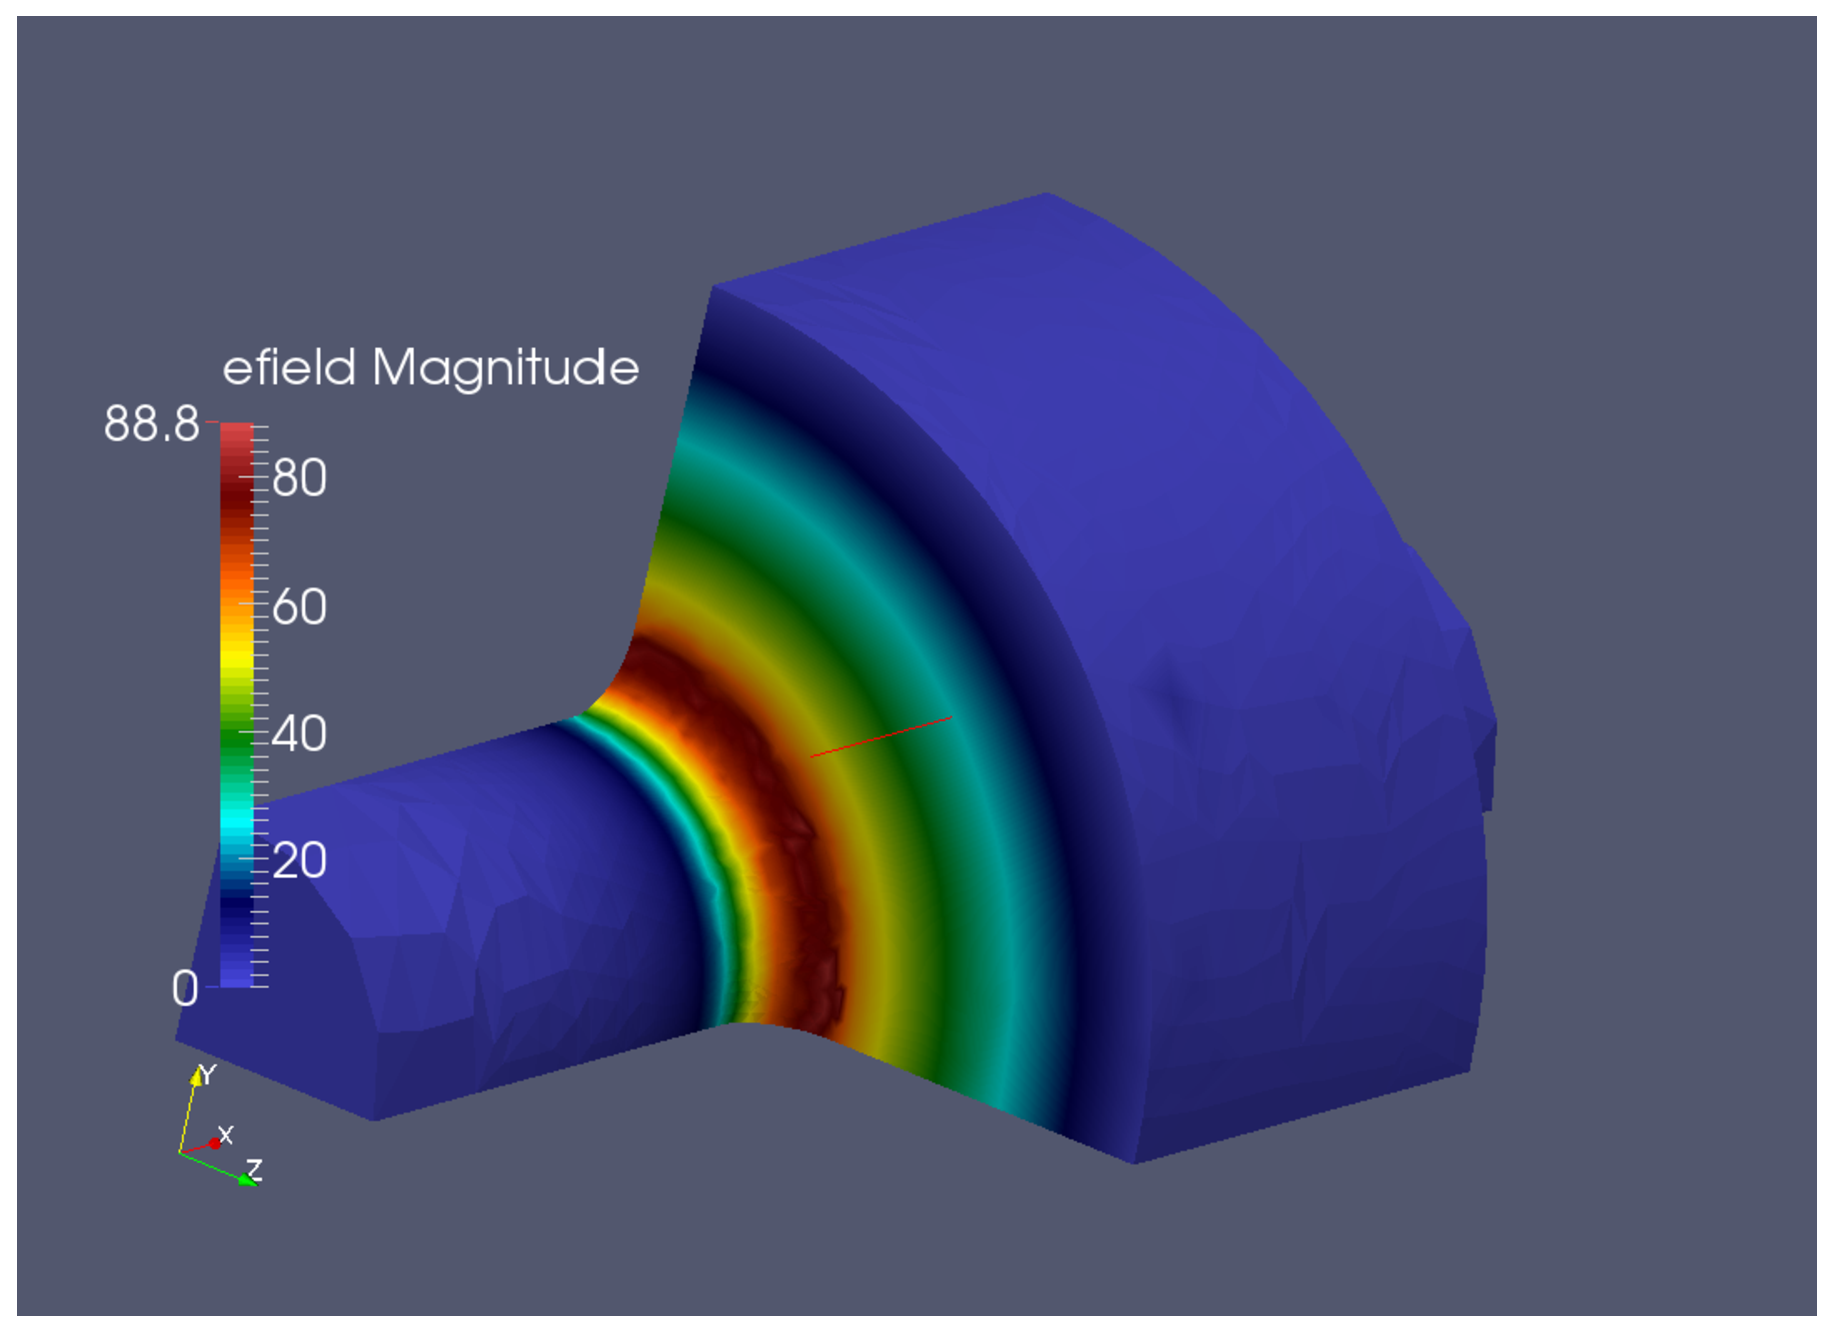
\includegraphics[width=0.49\textwidth]{figures/omega3p/pillbox_al_3_ar_0p0125_14221_elems_e_field.eps}
  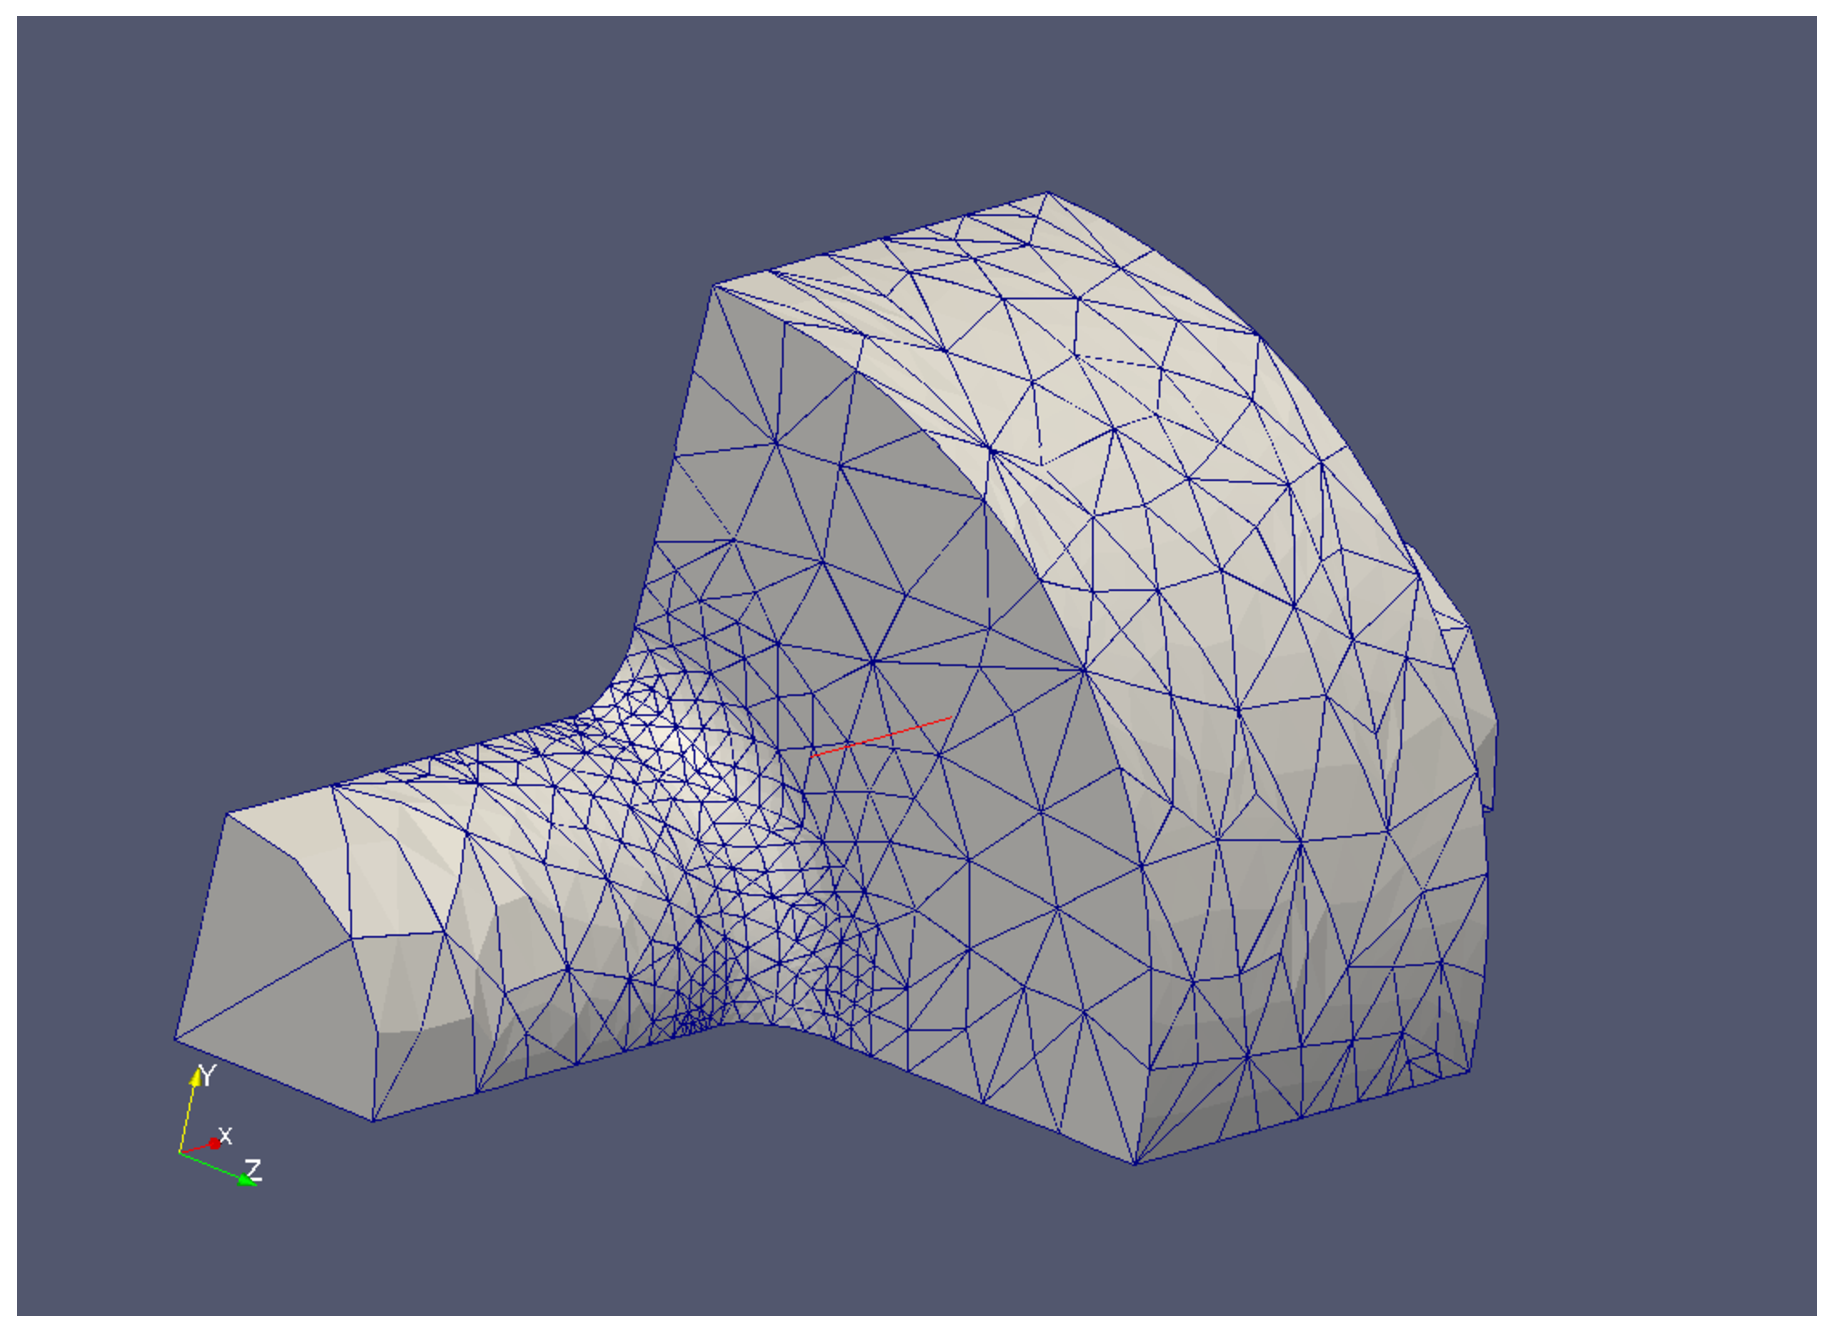
\includegraphics[width=0.49\textwidth]{figures/omega3p/pillbox_al_3_ar_0p0125_14221_elems_mesh.eps}
  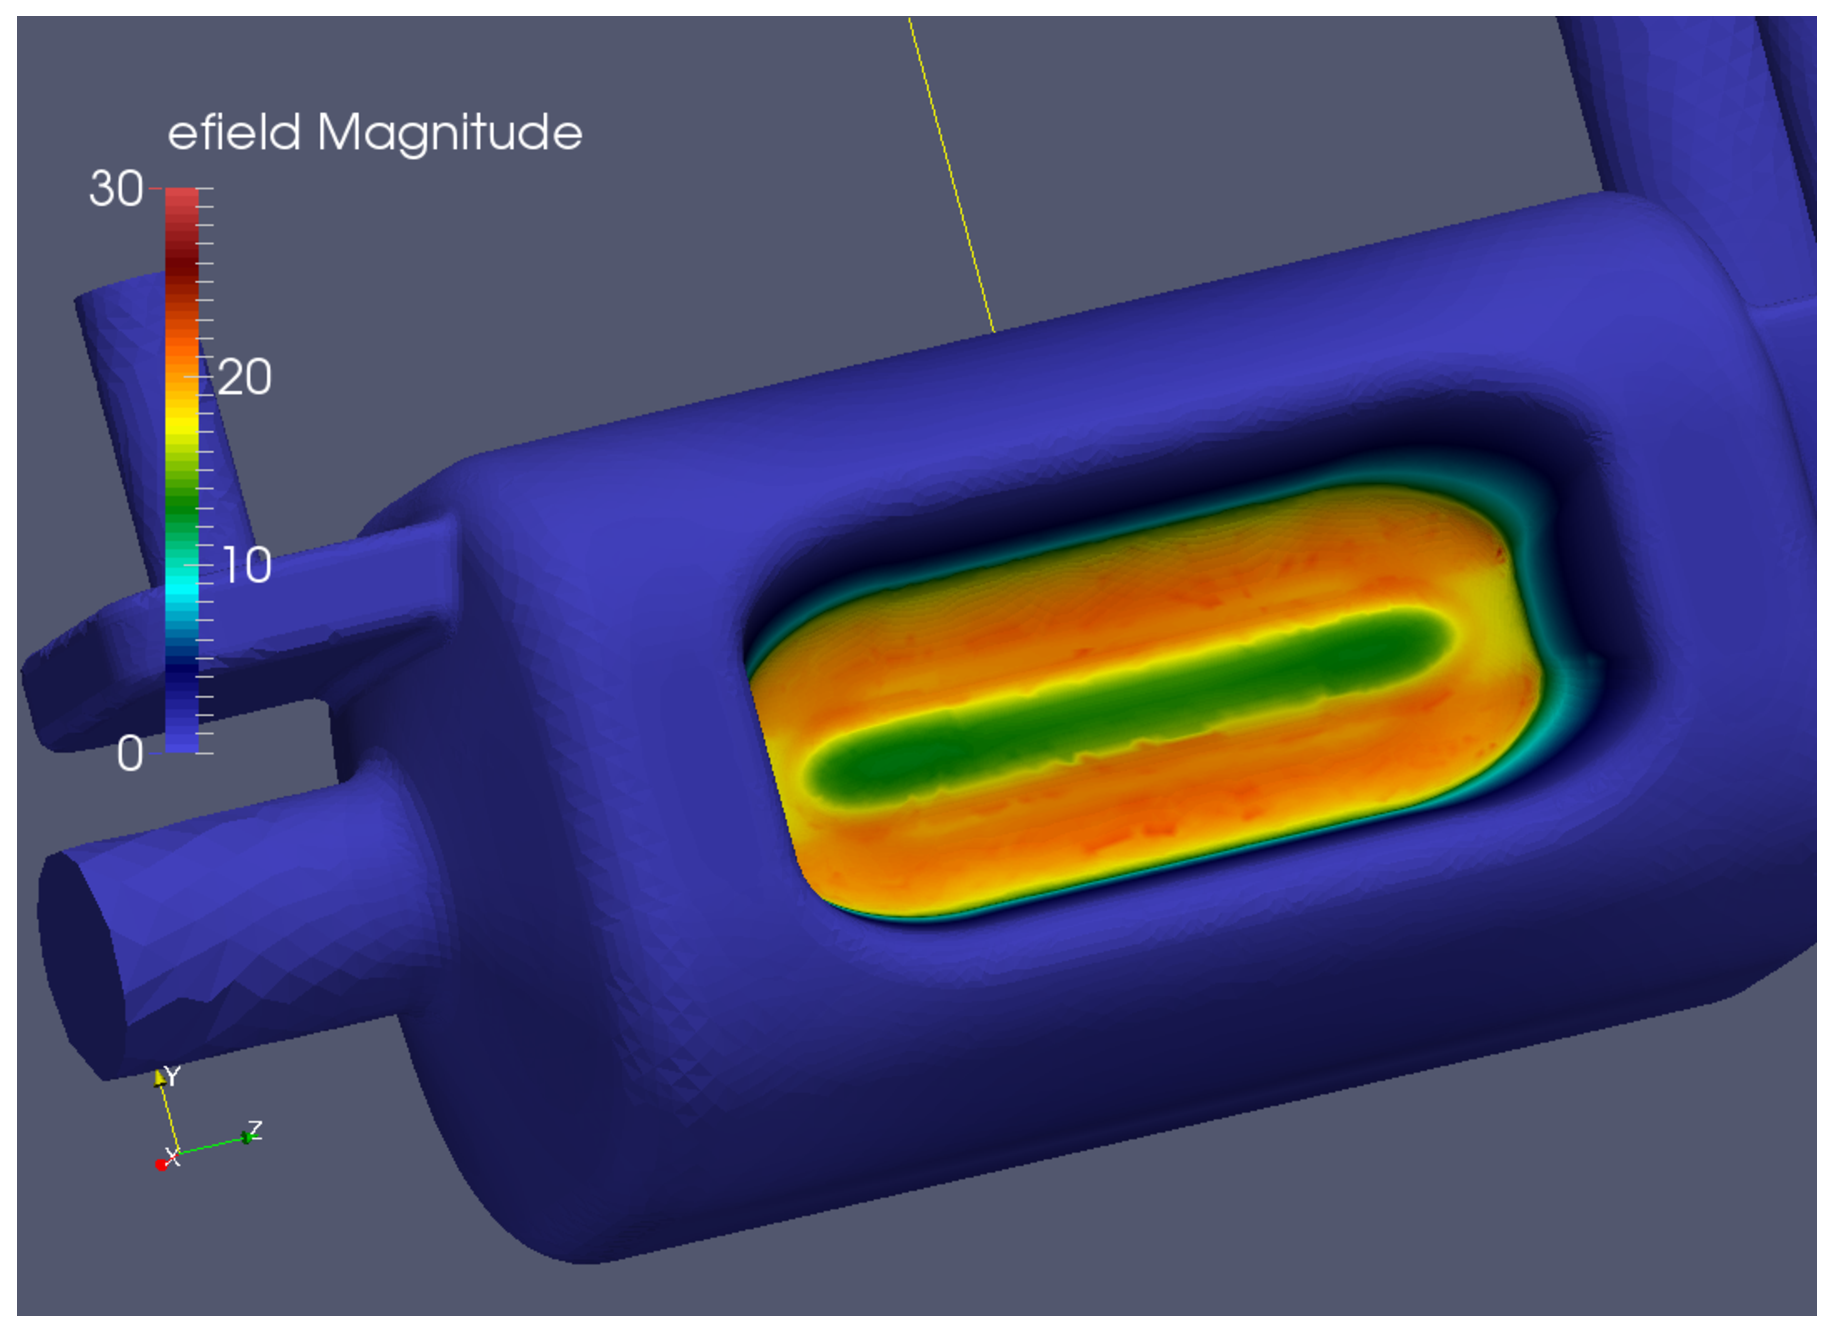
\includegraphics[width=0.49\textwidth]{figures/omega3p/cav17_al_3_ar_0p0125_386896_elems_e_field.eps}
  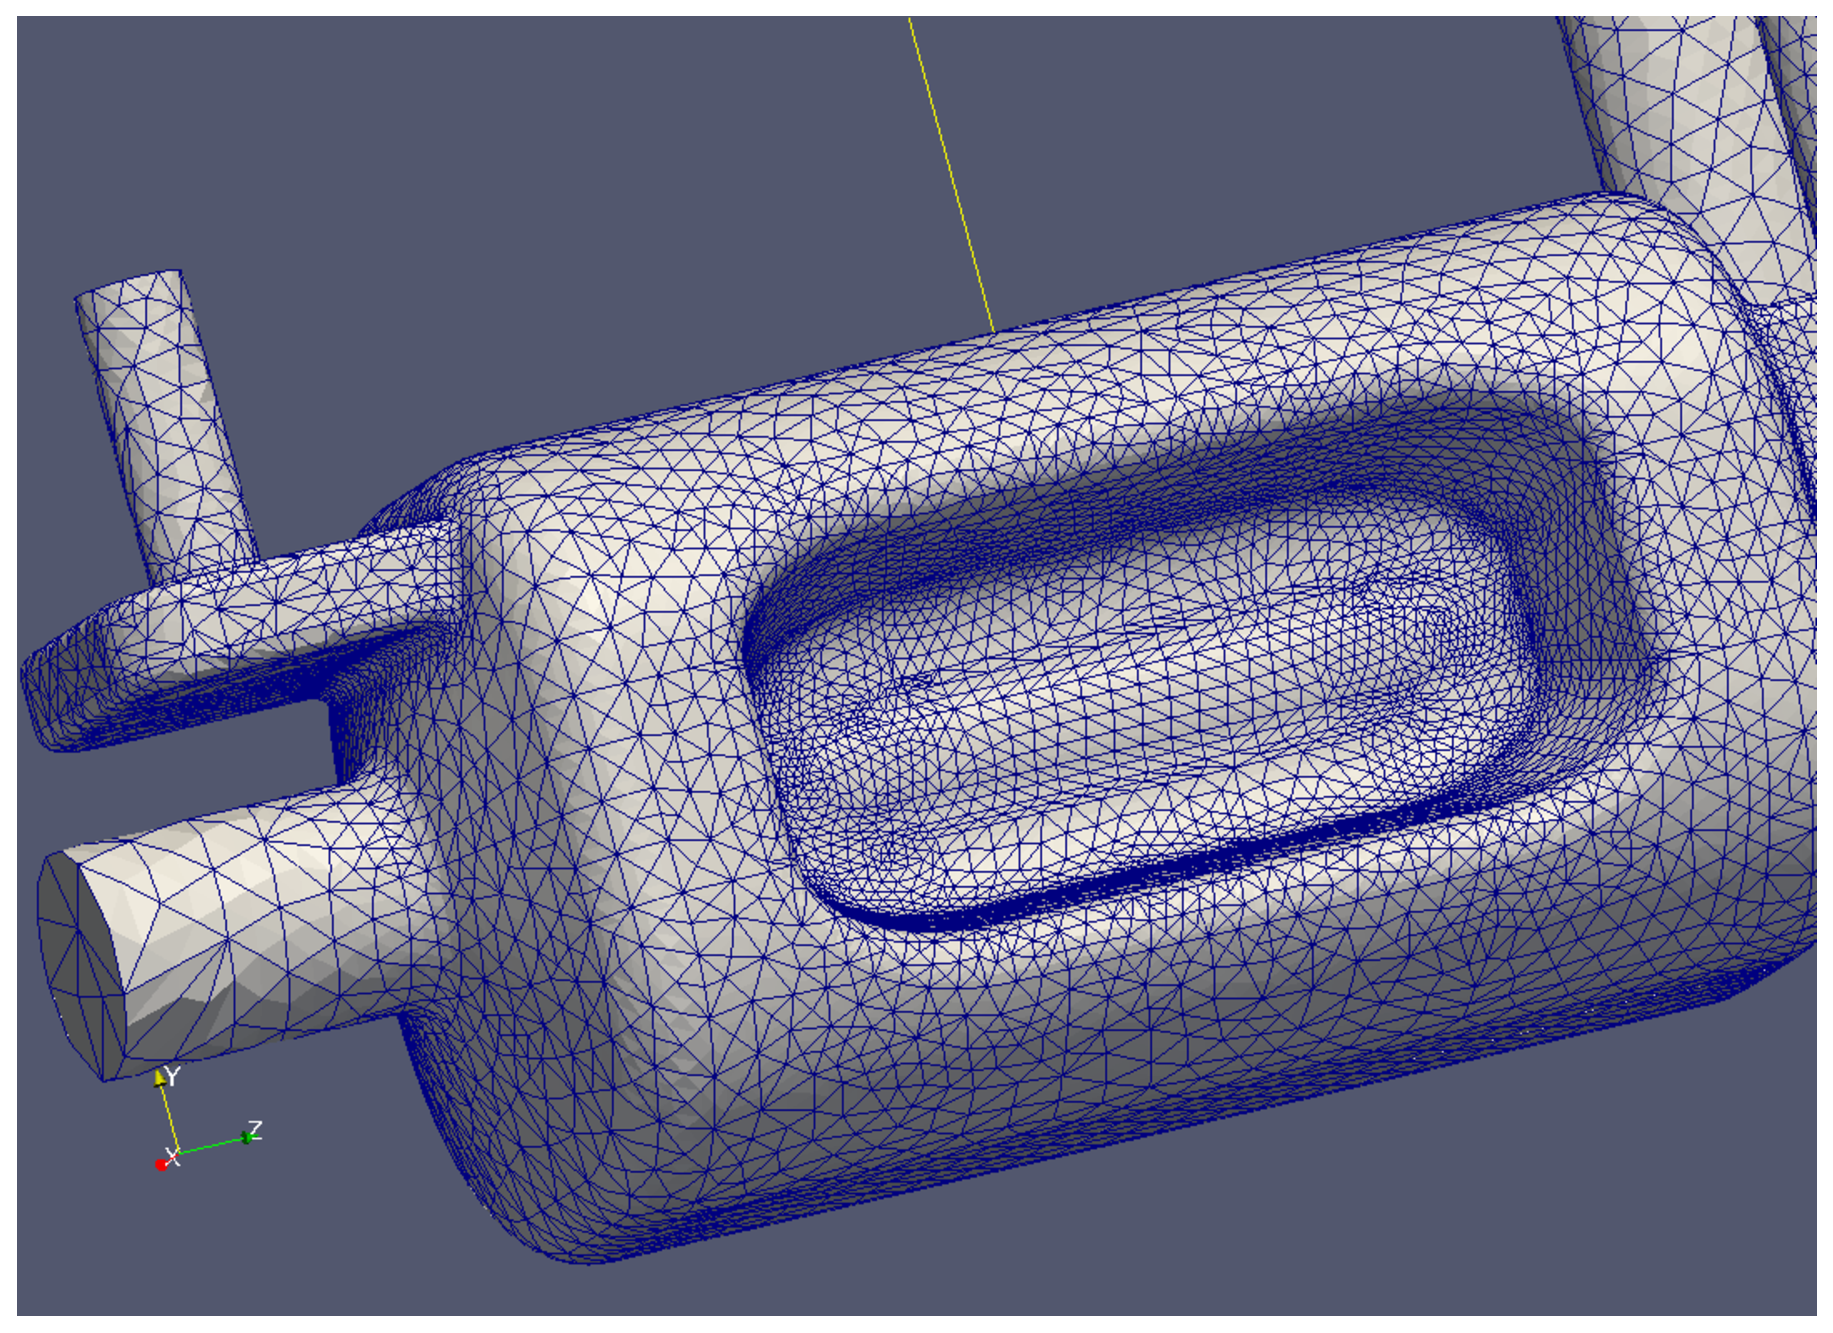
\includegraphics[width=0.49\textwidth]{figures/omega3p/cav17_al_3_ar_0p0125_386896_elems_mesh.eps}
  \caption{
    The first eigenmode electric field (left column) and adapted meshes
    (right column) for the \texttt{pillbox} (top row) and \texttt{cav17}
    (bottom row) test cases.
  }
  \label{fig:omega3pAdapt}
\end{figure}

The increase in peak memory usage from storing two copies of the mesh and
field data is insignificant relative to the applications
overall memory usage.
Fig.~\ref{fig:memusage} shows the peak per node memory usage over the entire
Omega3P execution on the \texttt{cav17} and \texttt{pillbox-2M} cases
for both the original Omega3P code and with the code that executes
PUMI mesh conversion and load balancing (Omega3P+PUMI).
As can be seen in the top half of Fig.~\ref{fig:memusage}, the \texttt{cav17}
model, the peak memory when storing the PUMI mesh increases by 2\% at 32 cores
and by 6\% at 128 cores, and decreases slightly at 64 cores (less than 1\%).
On the other hand, for the {\texttt pillbox-2M} case at 256, 512, and 1024
cores the peak memory is actually reduced by 0.87\%, 1.1\% and 2.9\%,
respectively.
The small reduction is the result of differences in the mesh loading and
balancing processes.
Specifically, at 256 processes ParMA balanced the mesh elements (owned and
ghosted) in the PUMI workflow to a 14\% imbalance while the non-PUMI workflow
using ParMETIS has a 38\% imbalance.
These results indicate that there is an insignificant memory overhead with the
in-memory integration process.

\begin{figure} [h] \centering
  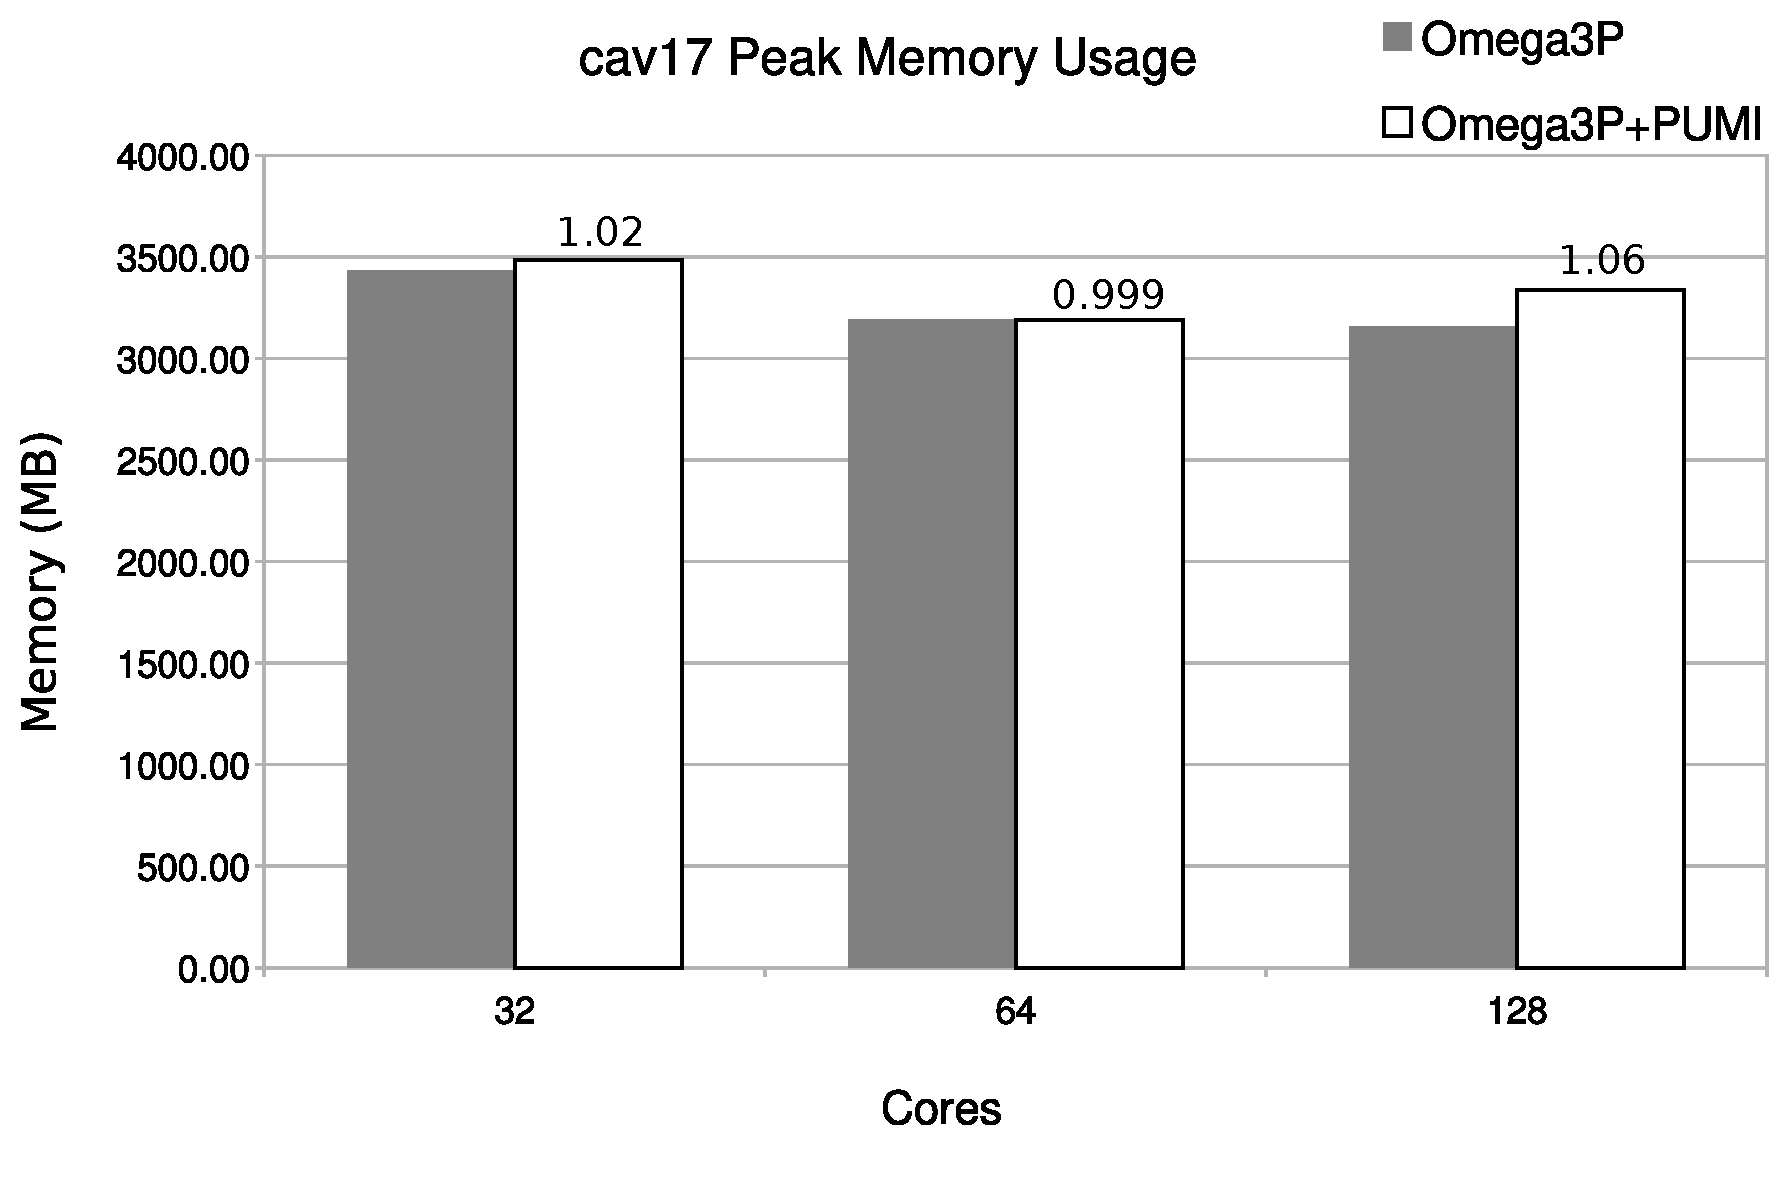
\includegraphics[width=.7\textwidth]{figures/omega3p/cav17-peak-mem.eps}
  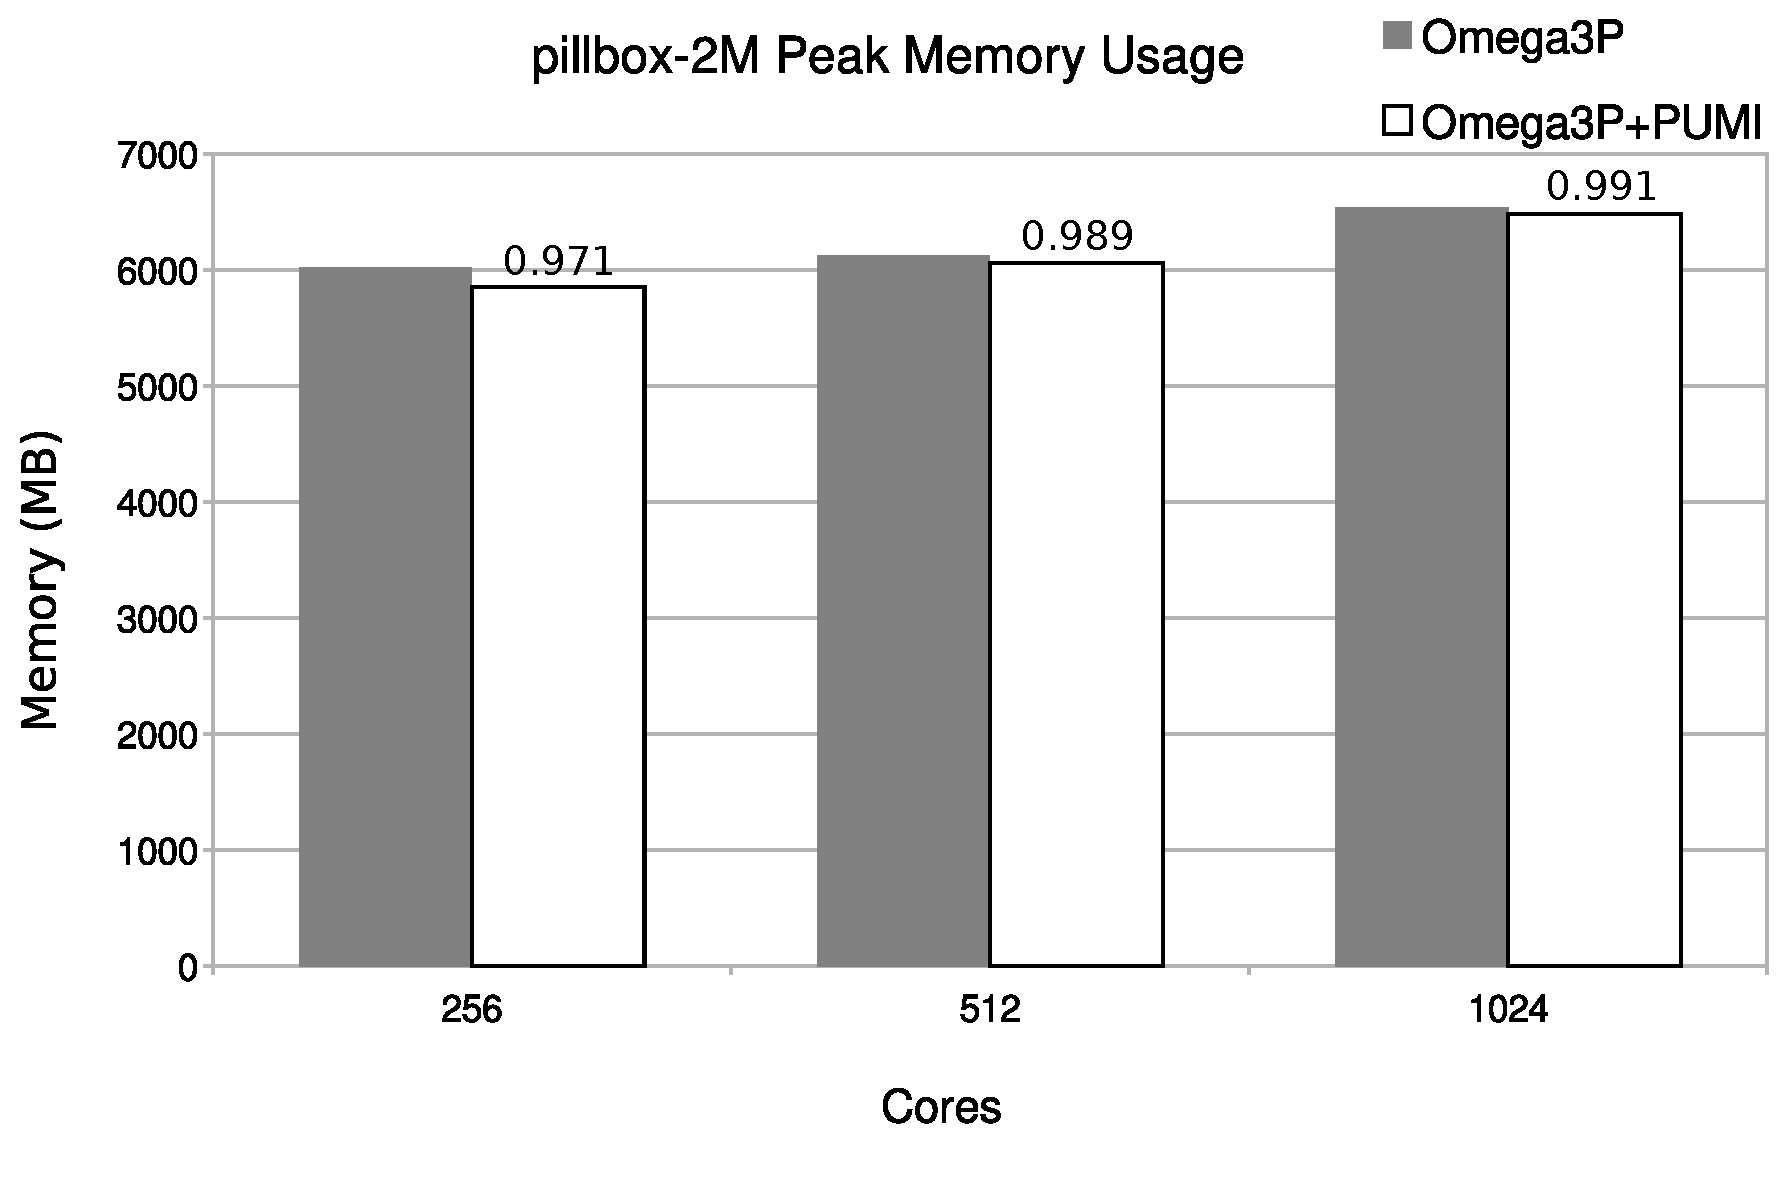
\includegraphics[width=.7\textwidth]{figures/omega3p/pillbox2M-peak-mem.eps}
  \caption[Peak per node memory usage for two Omega3P and Omega3P+PUMI test
           cases.]{
    Peak per node memory usage for two Omega3P and Omega3P+PUMI test cases:
    (top) {\texttt cav17} and (bottom) {\texttt pillbox-2M}.
    The numbers above the Omega3P+PUMI bars list the ratio of the peak memory
    used by Omega3P+PUMI relative to the peak memory used by Omega3P.
  }
  \label{fig:memusage}
\end{figure}
